% NOTE -- ONLY EDIT THE .Rnw FILE!!!  The .tex file is
% likely to be overwritten.
%
% \VignetteIndexEntry{clValid Overview}
% \VignetteDepends{cluster, kohonen, class, mclust, Biobase, annotate, GO, moe430a}
% \VignetteKeywords{clustering, validation, stability measures, biological annotation, functional categories}
% \VignettePackage{clValid}




\documentclass[11pt]{article}
%\documentclass[article, shortnames]{jss}

%\setlength{\oddsidemargin}{0.25truein}
%\setlength{\evensidemargin}{0.25truein}
%\setlength{\textwidth}{6.0truein} \setlength{\topmargin}{0.25truein}
%\setlength{\textheight}{8.5truein} \setlength{\headsep}{0.0truein}
%\setlength{\headheight}{0.0truein} \setlength{\topskip}{10.0pt}
%\pagestyle{empty} 
%\baselineskip=0.6cm

\usepackage{amsmath,amssymb,amsfonts} % Typical maths resource packages
\usepackage{graphics}                 % Packages to allow inclusion of graphics
\usepackage{color}                    % For creating coloured text and background
\usepackage{hyperref}                 % For creating hyperlinks in cross references
\usepackage{relsize}
\usepackage[mathcal]{euscript}
\usepackage[round]{natbib}
\usepackage{myCommands}
\usepackage{Sweave}
%\usepackage{Sweave}

%\usepackage{myCommands}
%\usepackage[round]{natbib}

%% need no \usepackage{Sweave}


\begin{document}

\author{Guy Brock, Vasyl
  Pihur, Susmita Datta, and Somnath Datta \\ \\
Department of Bioinformatics and Biostatistics, University of
Louisville \\
\url{http://louisville.edu/~g0broc01/} }

\title{\pkg{clValid}, an R package for cluster validation}

\maketitle

\tableofcontents

\begin{abstract}
The R package \pkg{clValid} contains functions for validating the results
of a clustering analysis.  There are three main types of cluster
validation measures available, ``internal'', ``stability'', and
``biological''.  
%The main function is \rf{clValid} ,and the available validation measures fall into the three general
%categories of ``internal'', ``stability'', and ``biological''.  
%Internal stability measures are based solely on the data, and consist
%of the connectivity 
The user can choose from nine clustering algorithms in
existing R packages, including
hierarchical, K-means, self-organizing maps (SOM), and model based clustering. 
In addition, we provide a function to perform the self-organizing tree
algorithm (SOTA) method of clustering.
Any combination of validation measures and
clustering methods can be requested in a single function call.  This allows the user to
simultaneously evaluate several clustering algorithms while varying
the number of clusters, to help determine the most appropriate method and
number of clusters for the dataset of interest.  
Additionally, the package can automatically make use of the biological
information contained in the Gene Ontology (GO) database to calculate
the biological validation measures, via the annotation packages
available in \href{http://www.bioconductor.org/}{Bioconductor}.
The function
returns an object of S4 class \rc{clValid}, which has summary, plot,
print, and additional methods which allow the user to display the optimal
validation scores and extract clustering results.  
\end{abstract}

%\Keywords{clustering, validation, R package, stability measures,
%  biological annotation, functional categories}


%\Address{
%Guy Brock\\
%Department of Bioinformatics and Biostatistics\\
%School of Public Health and Information Sciences\\
%University of Louisville\\
%555 S Floyd St.\\
%Louisville, KY, USA 40292\\
%E-mail: \email{guy.brock@louisville.edu}\\
%URL: \url{http://louisville.edu/~g0broc01/}
%}

%Telephone: 502-852-3444\\
%Fax: 502-852-3294\\





\section{Introduction}
\label{sec:introduction}

Clustering is an unsupervised technique used to group together objects which
are ``close'' to one another in a multidimensional feature space,
usually for the purpose of uncovering some inherent structure
which the data possesses.    
Clustering is commonly used in the
analysis of high-throughput genomic data, with the aim of 
grouping together genes or proteins which have similar
expression patterns and possibly share common biological pathways
\citep{DeR1997,Chu1998,Eis1998,Bha2007}. 
%One common example is microarray experiments, where genes or samples are grouped
%together on the basis of their similarity in expression profiles.  
A plethora of clustering algorithms currently exist, many of which
have shown some promise in the analysis of genomic data \citep{Her2001,McL2002,Dem2003,Fu2007}.  
Deciding which clustering method to use can therefore be a
daunting task for the researcher conducting the experiment.  
An additional, related problem is determining the number of clusters
that are most appropriate for the data.  Ideally, the resulting clusters should
not only have good statistical properties (compact, well-separated,
connected, and stable), but also
give results that are biologically relevant.


A variety of measures aimed at validating the
results of a clustering analysis and determining which clustering
algorithm performs the best for a particular experiment have been
proposed \citep{Ker2001, Yeu2001, Dat2003}.  This validation can be based solely on the internal properties
of the data or on some external reference, and on the expression data
alone or in conjunction with relevant biological information
\citep{Gib2002, Gat2003, Bol2005, Dat2006}.  The article by
\citet{Han2005}, in particular, gives an excellent overview of cluster
validation with post-genomic data and provides a synopsis of many of
the available validation measures. 


In this paper, we present an R package \pkg{clValid} which contains a
variety of methods for validating the results
from a clustering analysis.  
The main function is \rf{clValid()}, and the available validation measures fall into the three general
categories of ``internal'', ``stability'', and ``biological''.  
The user can simultaneously select multiple clustering algorithms,
validation measures, and numbers of clusters in a single function call,
to determine the most appropriate method and
an optimal number of clusters for the dataset.  
Additionally, the \pkg{clValid} package
makes use of the biological information contained in the 
\href{http://www.geneontology.org/}{Gene Ontology} 
(GO) database via the annotation packages
in \href{http://www.bioconductor.org/}{Bioconductor},
in order to automate the calculation of the biological validation measures.
The package also contains a function for implementing the
self-organizing tree algorithm (SOTA), which to our knowledge has not
been previously available in R packages on \href{http://www.r-project.org}{CRAN}.
The function
returns an object of S4 class \rc{clValid}, which has 
a variety of methods available to plot and summarize the validation
measures, display the optimal scores along with the corresponding cluster method
and number of clusters, and extract the clustering results for a
particular algorithm.


The rest of this paper is organized as follows.  Section \ref{sec:measures}
contains a detailed description of the validation measures that are
available.  Section \ref{sec:clustering} describes the clustering
algorithms which are available to use with the 
\pkg{clValid} package.  Section \ref{sec:illustration}
contain an example using mouse gene expression data from
\citet{Bha2007} that illustrates the use of the \pkg{clValid} package
functions and objects. Finally, Section \ref{sec:discussion} discusses
some additional validation software which is available, and some of
the benefits our software provides in comparison.



\section{Validation Measures}
\label{sec:measures}



The \pkg{clValid} package offers three types of cluster
validation, ``internal'', ``stability'', and ``biological''.  
Internal validation measures take only the dataset and the clustering
partition as input and use intrinsic information in the data to
assess the quality of the clustering.  
The stability measures are a special version of internal measures.
They evaluate the consistency of a clustering result by comparing it
with the clusters obtained after each column is removed, one at a time.
Biological validation evaluates the ability of a clustering algorithm
to produce biologically meaningful clusters.  We have measures
to investigate both the biological homogeneity and stability of the
clustering results.



\subsection{Internal measures}
\label{subsec:internal}


For internal validation, we selected measures that reflect the
compactness, connectedness, and separation of the cluster
partitions.  Connectedness relates to what extent observations are placed in the same
cluster as their nearest neighbors in the data space, and is here measured
by the connectivity \citep{Han2005}.  Compactness assesses cluster homogeneity, usually by
looking at the intra-cluster variance, while separation quantifies the
degree of separation between clusters (usually by measuring the
distance between cluster centroids).  Since compactness and separation
demonstrate opposing trends (compactness increases with the number of
clusters but separation decreases), popular methods combine the two
measures into a single score.  The Dunn Index \citep{Dun1974} and Silhouette
Width \citep{Rou1987} are
both examples of non-linear combinations of the compactness and
separation, 
and with the connectivity comprise the three internal measures
available in \pkg{clValid}.  The details of each measure are given
below, and for a good overview of internal measures in general see \citet{Han2005}.
%The measures
%included here are the 
%connectivity, and Silhouette Width, and the Dunn
%Index.  

\subsubsection*{Connectivity}

%The connectivity indicates the degree of connectedness of the
%clusters, i.e.~ 
Let $N$ denote the total number of observations (rows) in a dataset
and $M$ denote the total number of columns, which are assumed to be
numeric (e.g., a collection of samples, time points, etc.).
Define $nn_{i(j)}$ as the $j$th nearest neighbor of observation $i$, and
let $x_{i,nn_{i(j)}}$ be zero if $i$ and $j$ are in the same cluster and
$1/j$ otherwise.  Then, for a particular clustering partition
$\mathcal{C} = \{C_1, \ldots, C_K\}$ of the $N$ observations into $K$
disjoint clusters, the connectivity is defined as 
$$
Conn(\mathcal{C}) = \sum\limits_{i=1}^N\sum\limits_{j=1}^M x_{i,nn_{i(j)}} \;.
$$
The connectivity has a value between zero and $\infty$ and should be minimized.
%The \code{neighbSize} argument to \rf{clValid()} specifies the number of
%neighbors to use for the connectivity measure.

\subsubsection*{Silhouette Width}

The Silhouette Width is the average of each observation's Silhouette
value.
The Silhouette value  measures the
degree of confidence in the clustering assignment of a particular
observation, with
well-clustered observations having values
near $1$ and poorly clustered observations having values near $-1$.  For
observation $i$, it is defined as
$$ 
S(i) = \frac{b_i - a_i}{max(b_i, a_i)}\,,
$$
where $a_i$ is the average distance between $i$ and all other
observations in the same cluster, and $b_i$ is the average distance
between $i$ and the observations in the ``nearest neighboring
cluster'', i.e. % (which is defined as the cluster mininizing )
$$
b_i = \min\limits_{C_k \in \mathcal{C}\setminus C(i)} \sum\limits_{j \in C_k}\frac{dist(i,j)}{n(C_k)}\,,
$$
where $C(i)$ is the cluster containing observation $i$, $dist(i,j)$ is
the distance (e.g.~Euclidean, Manhattan) between observations $i$ and $j$, and $n(C)$ is the
cardinality of cluster $C$.  The Silhouette Width thus lies in the interval
$[-1,1]$, and should be maximized.  
For more information, see the help page for the \rf{silhouette()}
function in package \pkg{cluster} \citep{cluster}.
% for more details.  

\subsubsection*{Dunn Index}

The Dunn Index is the ratio of the smallest distance between
observations not in the same cluster to the largest intra-cluster
distance.  It is computed as 
$$
D(\mathcal{C}) = \frac{\min\limits_{C_k, C_l \in \mathcal{C}, \,C_k
    \neq C_l} \left(\min\limits_{i\in C_k, \,j\in C_l} dist(i,j)\right)}{\max\limits_{C_m \in \mathcal{C}}
    diam(C_m)} \,,
$$
where $diam(C_m)$ is the maximum distance between observations in
cluster $C_m$.
%, and $dist(C_k, C_l)$ is the minimal distance between 
%pairs of observations $i$ and $j$ with $i$ in $C_k$ and $j$ in $C_l$.  
The Dunn Index has a value between zero and $\infty$, and should be maximized.

%For further details on all the aforementioned measures refer to 



\subsection{Stability measures}
\label{subsec:stability}

The stability measures compare the results from clustering based on
the full data to clustering based on removing each column, one at a time.
These measures work especially well if the data are highly
correlated, which is often the case in high-throughput genomic data. 
The included measures are the average proportion of non-overlap (APN),
the average distance (AD), the average distance between means (ADM),
and the figure of merit (FOM) \citep{Dat2003, Yeu2001}.    
In all cases the average is taken over all the
deleted columns, and all measures should be minimized.  

\subsubsection*{Average Proportion of Non-overlap (APN)}

%The APN, AD, and ADM are all based on the
%cross-classification table of the the original clustering with the
%clustering based on the removal of one column.  
The APN measures the average proportion of observations not placed in the
same cluster by clustering based on the full data and clustering based
on the data with a single column removed.  
Let $C^{i,0}$ represent the cluster
containing observation $i$ using the original clustering (based on all available
data), and $C^{i,\ell}$ represent the cluster containing observation
$i$ where the clustering is based on the dataset with column $\ell$
removed.  %Also, let $n(C)$ indicate the cardinality of cluster $C$.  
Then, with the total number of clusters set to $K$, the
APN measure is defined as 
$$
APN(K) = \frac{1}{MN}\sum\limits_{i=1}^N\sum\limits_{\ell=1}^M \left( 1 -
  \frac{n(C^{i,\ell} \cap C^{i,0})}{n(C^{i,0})} \right) \,.
$$
The APN is in the interval $[0,1]$, with values close to zero
corresponding with highly consistent clustering results.

\subsubsection*{Average Distance (AD)}

The AD measure computes the average distance between observations placed
in the same cluster by clustering based on the full data and clustering based
on the data with a single column removed.  
It is defined as 
$$
AD(K) = \frac{1}{MN}\sum\limits_{i=1}^N\sum\limits_{\ell=1}^M
\frac{1}{n(C^{i,0})n(C^{i,\ell})}\left[ \sum\limits_{i\in C^{i,0}, j
  \in C^{i,\ell}} dist(i,j)\right] \,.
$$
The AD has a value between zero and $\infty$, and smaller values are preferred.

\subsubsection*{Average Distance between Means (ADM)}
The ADM measure computes  the average
distance between cluster centers for observations placed in the same cluster
by clustering based on the full data and clustering based
on the data with a single column removed.  
It is defined as 
$$
ADM(K) =  \frac{1}{MN}\sum\limits_{i=1}^N\sum\limits_{\ell=1}^M
dist(\bar{x}_{C^{i,\ell}}, \bar{x}_{C^{i,0}})\,,
$$
where $\bar{x}_{C^{i,0}}$ is the mean of the observations in the
cluster which contain observation $i$, when clustering is based on the
full data, and $\bar{x}_{C^{i,\ell}}$ is similarly defined.
Currently, ADM only uses the Euclidean distance. % (is this true??). 
It also has a value between zero and $\infty$, and again smaller
values are prefered.

\subsubsection*{Figure of Merit (FOM)}

The FOM measures the average intra-cluster variance
of the observations in the deleted column, where the clustering is based on the remaining
(undeleted) samples.  This estimates the mean error using
predictions based on the cluster averages.
For a particular left-out column $\ell$, the FOM is 
$$
FOM(\ell, K) =  \sqrt{\frac{1}{N}\sum\limits_{k=1}^K\sum\limits_{i\in
    C_k(\ell)} dist(x_{i,\ell}, \bar{x}_{C_k(\ell)})}\,,
$$
where $x_{i,\ell}$ is the value of the $i$th observation in the
$\ell$th column in
cluster $C_k(\ell)$, and $\bar{x}_{C_k(\ell)}$ is the average of
cluster ${C_k(\ell)}$.
Currently, the only distance available for FOM is Euclidean.
The FOM is multiplied by an adjustment factor $\sqrt{\frac{N}{N-K}}$,
to alleviate the tendency to decrease as the number of clusters
increases.  The final score is averaged over all the removed columns,
and has a value between zero and $\infty$, with smaller values
equaling better performance. 
%The FOM should be minimized.



\subsection{Biological}
\label{subsec:biological}

Biological validation evaluates the ability of a clustering algorithm
to produce biologically meaningful clusters.  A typical application of
biological validation is in microarray data, where observations
correspond to genes (where ``genes'' could be open reading frames
(ORFs), express sequence tags (ESTs), serial analysis of gene
expression (SAGE) tags,
etc.).  There are two measures available, the biological homogeneity index (BHI) and
biological stability index (BSI), both originally presented in \citet{Dat2006}.  

\subsubsection*{Biological Homogeneity Index (BHI)}

As its name implies, the BHI
measures how homogeneous the clusters are biologically.  
Let $\mathcal{B} = \{B_1, \ldots, B_F\}$ be a set of $F$ functional
classes, not necessarily disjoint, and let $B(i)$ be the functional
class containing gene $i$ (with possibly more
than one functional class containing $i$).  Similarly, we define
$B(j)$ as the function class containing gene $j$, and assign the
indicator function $I(B(i) = B(j))$ the value $1$ if $B(i)$ and $B(j)$
match (any one match is sufficient in the case of membership to
multiple functional classes), and 0 otherwise.  Intuitively, we hope that genes placed
in the same statistical cluster also belong to the same functional
classes.  Then, for a given statistical clustering
partition $\mathcal{C} = \{C_1, \ldots, C_K\}$ and set of biological
classes $\mathcal{B}$, the BHI is defined as 
$$
BHI(\mathcal{C},\mathcal{B}) = \frac{1}{K} \sum\limits_{k=1}^K
\frac{1}{n_k(n_k-1)} \sum\limits_{i\neq j \in C_k} I\left(B(i)=B(j)\right)\,.
$$
Here $n_k = n(C_k \cap B)$ is the number of annotated genes in
statistical cluster $C_k$. The BHI is in the range $[0,1]$, with
larger values corresponding to more biologically homogeneous clusters.

\subsubsection*{Biological Stability Index (BSI)}

The BSI is similar to the other stability
measures, and inspects the consistency of clustering for genes with
similar biological functionality.  Each sample is removed one at a
time, and the cluster membership for genes with similar functional annotation
is compared with the cluster membership using all available samples.
The BSI is defined as 
$$
BSI(\mathcal{C}, \mathcal{B}) = \frac{1}{F}\sum\limits_{k=1}^F
\frac{1}{n(B_k)(n(B_k)-1)M} \sum\limits_{\ell=1}^M \sum\limits_{i\neq j\in
    B_k} \frac{n(C^{i,0} \cap C^{j,\ell})}{n(C^{i,0})}\,,
$$
where $F$ is the total number of functional classes, $C^{i,0}$ is the statistical cluster containing observation $i$
based on all the data, and $C^{j,\ell}$ is the statistical cluster
containing observation $j$ when column $\ell$ is removed.  The BSI is
in the range $[0,1]$, with larger values corresponding to more stable
clusters of the functionally annotated genes.

%The BSI 
%computes the average overlap of statistical clusters
%  based on all the samples with that based on all but one sample for genes
%  that are placed in the same functional class.

%The BHI measures the average
%  proportion of gene pairs with matching functional classes that are
%  clustered together. 




\section{Clustering Algorithms}
\label{sec:clustering}

The R statistical computing project \citep{R} has a wide variety of
clustering algorithms available in the base distribution and various
add-on packages.  We make use of nine algorithms from the base
distribution and add-on packages \pkg{cluster} \citep{cluster, Kau1990}, \pkg{kohonen} \citep{kohonen}, and
\pkg{mclust} \citep{mclust, Fra2003}, and in addition provide a function for implementing
SOTA in the \pkg{clValid} package.
A brief description of each clustering method and its availability is
given below.



\subsubsection*{UPGMA}

Unweighted Pair Group Method with Arithmetic Mean is probably the most
frequently used clustering algorithm \citep{Kau1990}.   It is an agglomerative,
hierarchical clustering algorithm that yields a dendogram which can
be cut at a chosen height to produce the desired number of clusters.
Each observation is initially placed in its own cluster, and the clusters are
successively joined together in order of their ``closeness''.  The
closeness of any two clusters is determined by a dissimilarity
matrix, and can be based on a variety of agglomeration methods.  
UPGMA is included with the base distribution of R in function
\rf{hclust()}, and is also implemented in the \rf{agnes()}
function in package \pkg{cluster}.


\subsubsection*{K-means}
K-means is an iterative method which minimizes the within-class sum of
squares for a given number of clusters \citep{Har1979}.  The algorithm starts with an
initial guess for the cluster centers, and each observation is placed
in the cluster to which it is closest.  The cluster centers are then
updated, and the entire process is repeated until the cluster centers
no longer move.  Often another clustering algorithm (e.g., UPGMA) is run initially to
determine starting points for the cluster centers.  K-means is
implemented in the function \rf{kmeans()}, included with the base
distribution of R.
  
\subsubsection*{Diana}
Diana is a divisive hierarchical algorithm that initially starts with
all observations in a single cluster, and successively divides the
clusters until each cluster contains a single observation.  
Along with SOTA, Diana is one of a few representatives of the divisive hierarchical approach
to clustering.  Diana is available in function \rf{diana()} in package \pkg{cluster}.


\subsubsection*{PAM}
Partitioning around medoids (PAM) is similar to K-means, but is considered more
robust because it admits the use of other dissimilarities besides
Euclidean distance.  Like K-means, the number of clusters is fixed in
advance, and an initial set of cluster centers is required to start
the algorithm.  PAM is available in the \pkg{cluster} package as
function \rf{pam()}.

\subsubsection*{Clara}
Clara is a sampling-based algorithm which implements PAM
on a number of sub-datasets \citep{Kau1990}. This allows for faster
running times when a number of observations is relatively large.
Clara is also available in package \pkg{cluster} as function \rf{clara()}.


\subsubsection*{Fanny}
This algorithm performs fuzzy clustering, where each observation can
have partial membership in each cluster \citep{Kau1990}. Thus, each
observation has a vector which gives the partial membership to each of
the clusters.  
A hard cluster can be produced by assigning each observation to the
cluster where it has the highest membership.  Fanny is available in
the \pkg{cluster} package (function \rf{fanny()}).


\subsubsection*{SOM}
Self-organizing maps \citep{Koh1997} is an unsupervised learning
technique that is popular among computational biologists and
machine learning researchers.  SOM is based on neural
networks,
and is highly regarded for its ability to
map and visualize high-dimensional data in two dimensions.
SOM is available as the \rf{som()} function in package \pkg{kohonen}.


\subsubsection*{Model based clustering}
Under this approach, a statistical model consisting of
a finite mixture of Gaussian distributions is fit to the
data  \citep{Fra2001}. 
Each mixture component represents a cluster, and the mixture
components and group memberships are estimated using 
maximum likelihood (EM algorithm).
The function \rf{Mclust()} in package \pkg{mclust} implements model
based clustering.
%The number of clusters and the Gaussian models are
%chosen by the minimum BIC criterion.


\subsubsection*{SOTA}
Self-organizing tree algorithm (SOTA) is an unsupervised
network with a divisive hierarchical binary tree structure. 
%It combines
%the advantages of both hierarchical clustering and SOM.
It was originally proposed by \citet{Dop1997} for phylogenetic
reconstruction, and later applied to cluster microarray gene
expression data in \citep{Her2001}. 
It uses a fast algorithm and hence is suitable
for clustering a large number of objects.
SOTA is included with the \pkg{clValid} package as function \rf{sota()}.





\section{Example - Mouse Mesenchymal Cells}
\label{sec:illustration}

To illustrate the cluster validation measures in package
\pkg{clValid}, we use data from an Affymetrix microarray experiment
comparing gene expression of mesenchymal cells from two distinct
lineages, neural crest and mesoderm-derived.  The dataset consists of
147 genes and ESTs which were determined to
be significantly differentially expressed between the two cell lineages,
with at least a 1.5 fold increase or decrease in expression.  There
are three samples for each of the neural crest and mesoderm-derived
cells, so the expression matrix has dimension $147\times 6$.  In
addition, the genes were grouped into the functional classes according
to their biological description, with categories ECM/receptors (16),
growth/differentiation (16), kinases/phosphatases (7), metabolism (8),
stress-induced (6), transcription factors (28), and miscellaneous
(25).  The biological function of 10 genes was unknown, and 31 of the
``genes'' were ESTs.
For further description of the dataset and the experiments the reader is referred to \citet{Bha2007}.

%NOTE1: It takes some time (several minutes) to run the code for this
%example.  Run times can be reduced by removing some of the clustering
%methods from the validation.

NOTE: The clValid package uses package \pkg{mclust}, see the note
below for usage.


\begin{Schunk}
\begin{Soutput}
use of mclust requires a license agreement
see http://www.stat.washington.edu/mclust/license.txt
\end{Soutput}
\end{Schunk}

We begin by loading the dataset:
\begin{Schunk}
\begin{Sinput}
> data(mouse)
\end{Sinput}
\end{Schunk}
This dataset has the typical format found in  microarray
data, with the rows as genes (variables) and the columns as the
samples. 
% Although this is a common paradigm for those who routinely
% analyze high throughput genomic data, 
Although this is a transposition of the data structure used for more
conventional statistics (rows are samples, columns are variables),
in both cases the typical goal is to cluster the rows based on the
columns (although, in microarray data analysis the samples are also
commonly clustered).  Hence, the \rf{clValid} function assumes that
the rows of the input matrix are the intended items to be clustered.

We want to evaluate the results from a clustering analysis, using the
clustering algorithms UPGMA, PAM, and K-means.   Since the genes fall
into one of two groups, up or down-regulated in the neural
crest vs.~mesoderm-derived tissue, the numbers of clusters is varied
from 2 to 6.  The distance metric (both for the applicable
clustering methods and validation measures) is set to ``euclidean''; other available options are
``correlation'' and ``manhattan''.  The agglomeration method for
hierarchical clustering is set to ``average''.  
We illustrate each category of validation measure separately, but it
should be noted that the user can request all three types of
validation measures at once (which would also be more computationally efficient).


\subsubsection*{Internal Validation}

The internal validation measures are the connectivity, Silhouette Width, and
Dunn Index.   The neighborhood size for the connectivity is
set to 10 by default, the \rfarg{neighbSize} argument can be used to change
this.  Note that the clustering method ``agnes'' was omitted, since
this also performs hierarchical clustering and would be redundant with
the ``hierarchical'' method.  

\begin{Schunk}
\begin{Sinput}
> express <- mouse[, c("M1", "M2", "M3", "NC1", "NC2", "NC3")]
> rownames(express) <- mouse$ID
> intern <- clValid(express, 2:6, clMethods = c("hierarchical", 
+     "kmeans", "pam"), validation = "internal")
\end{Sinput}
\end{Schunk}

To view the results of the analysis, print, plot, and summary methods
are available for the \ro{clValid} object \ro{intern}.  The summary
statement will display all the validation measures in a table, and
also give the clustering method and number of clusters corresponding
to the optimal score for each measure.

\begin{Schunk}
\begin{Sinput}
> summary(intern)
\end{Sinput}
\begin{Soutput}
Clustering Methods:
 hierarchical kmeans pam 

Cluster sizes:
 2 3 4 5 6 

Validation Measures:
                                 2       3       4       5       6
                                                                  
hierarchical Connectivity   5.3270 14.2528 20.7520 27.0726 30.6194
             Dunn           0.1291  0.0788  0.0857  0.0899  0.0899
             Silhouette     0.5133  0.4195  0.3700  0.3343  0.3233
kmeans       Connectivity  13.2548 17.6651 37.3980 43.2655 50.6095
             Dunn           0.0464  0.0873  0.0777  0.0815  0.0703
             Silhouette     0.4571  0.4182  0.3615  0.3367  0.3207
pam          Connectivity  18.7917 27.9651 30.9302 44.9671 32.9667
             Dunn           0.0391  0.0597  0.0510  0.0761  0.0816
             Silhouette     0.4271  0.3489  0.3563  0.3530  0.4152

Optimal Scores:

             Score  Method       Clusters
Connectivity 5.3270 hierarchical 2       
Dunn         0.1291 hierarchical 2       
Silhouette   0.5133 hierarchical 2       
\end{Soutput}
\end{Schunk}

Hierarchical clustering with two clusters performs the best in each
case.  The validation measures can also be displayed graphically using
the \rf{plot()} method.  Plots for individual measures can be requested
using the \rfarg{measures} argument.  A legend is also included with each plot.  The default location of the
legend is the top right corner of each plot, this can be changed using
the \rfarg{legendLoc} argument.  Here, we combine all three plots into
a single figure and so suppress the legends in each individual plot.



\begin{Schunk}
\begin{Sinput}
> op <- par(no.readonly = TRUE)
> par(mfrow = c(2, 2), mar = c(4, 4, 3, 1))
> plot(intern, legend = FALSE)
> plot(nClusters(intern), measures(intern, "Dunn")[, , 1], type = "n", 
+     axes = F, xlab = "", ylab = "")
> legend("center", clusterMethods(intern), col = 1:9, lty = 1:9, 
+     pch = paste(1:9))
> par(op)
\end{Sinput}
\end{Schunk}

\begin{figure}
  \centering
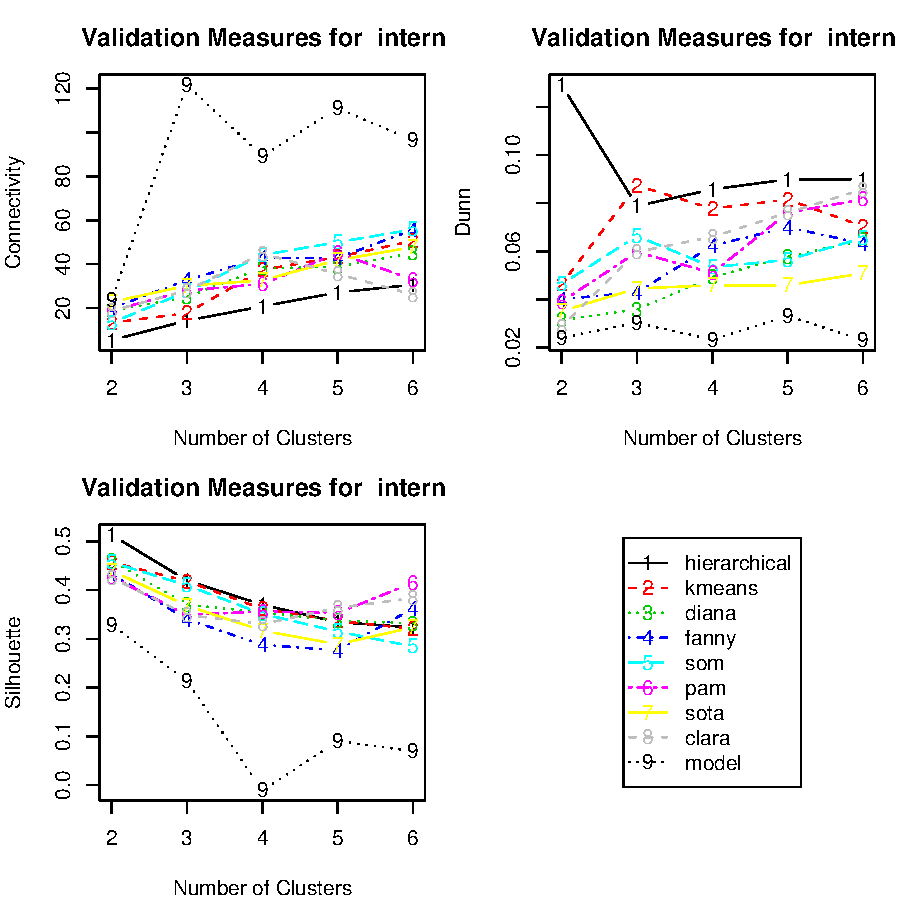
\includegraphics{clValid-006}
  \caption{Plots of the connectivity measure, the Dunn Index, and the
    Silhouette Width.}
  \label{fig:internPlot}
\end{figure}


The plots of the connectivity, Dunn Index, and Silhouette Width are given in 
Figure \ref{fig:internPlot}.
%Figures \ref{fig:conn}, \ref{fig:dunn}, and \ref{fig:sil}, respectively.  
Recall that the connectivity should be minimized, while both the Dunn
Index and the Silhouette Width should be maximized.  Thus, it appears
that hierarchical clustering (UPGMA) 
outperforms the other clustering algorithms under each validation
measure.
For hierarchical clustering the optimal number of clusters is clearly
two.  For PAM, a case could be made for using six clusters.


\subsubsection*{Stability Validation}

The stability measures include the APN, AD, ADM, and FOM.  The
measures should be minimized in each case.  Stability validation
requires more time than internal validation, since clustering needs to
be redone for each of the datasets with a single column removed.  

\begin{Schunk}
\begin{Sinput}
> stab <- clValid(express, 2:6, clMethods = c("hierarchical", "kmeans", 
+     "pam"), validation = "stability")
\end{Sinput}
\end{Schunk}

Instead of viewing all the validation measures via the \rf{summary()}
method, we can instead just view the optimal values using the
\rf{optimalScores()} method.

\begin{Schunk}
\begin{Sinput}
> optimalScores(stab)
\end{Sinput}
\begin{Soutput}
         Score       Method Clusters
APN 0.04781010 hierarchical        2
AD  1.52717887          pam        6
ADM 0.14007952          pam        6
FOM 0.51580323          pam        6
\end{Soutput}
\end{Schunk}

For the APN measures, hierarchical clustering with two
clusters again gives the best score.  However, for the other three
measures PAM with six clusters has the best score.  It
is illustrative to graphically visualize each of the validation
measures.  The plot of the FOM measure is very similar to the AD measure, so we
have omitted it from the figure.

% omit FOM - very similar to AD


\begin{Schunk}
\begin{Sinput}
> par(mfrow = c(2, 2), mar = c(4, 4, 3, 1))
> plot(stab, measure = c("APN", "AD", "ADM"), legend = FALSE)
> plot(nClusters(stab), measures(stab, "APN")[, , 1], type = "n", 
+     axes = F, xlab = "", ylab = "")
> legend("center", clusterMethods(stab), col = 1:9, lty = 1:9, 
+     pch = paste(1:9))
> par(op)
\end{Sinput}
\end{Schunk}

\begin{figure}
  \centering
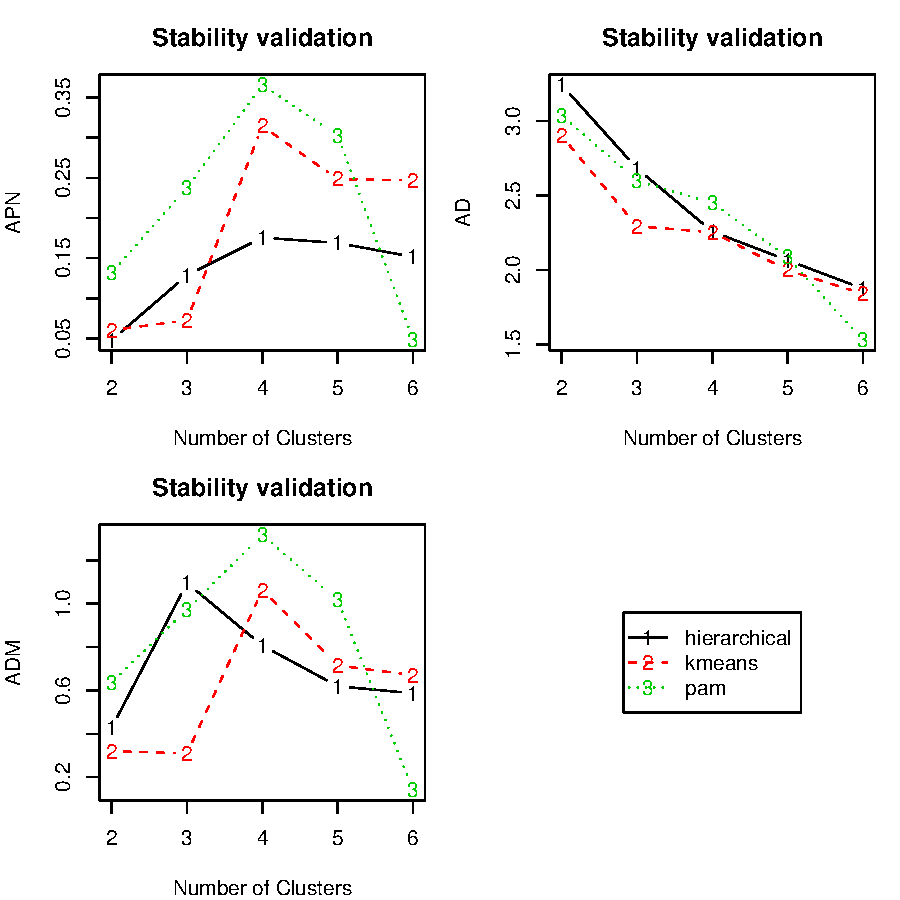
\includegraphics{clValid-010}
  \caption{Plot of the APN, AD, and APN  measures.}
  \label{fig:stabPlot}
\end{figure}

%   \includegraphics[height=6in,width=6in]{"clValidPaper-stabPlot"}


The plots of the APN, AD, and ADM are given in Figure
\ref{fig:stabPlot}.
%\ref{fig:APN}, \ref{fig:AD}, \ref{fig:ADM}, \ref{fig:FOM}, respectively.  
The APN measure shows an interesting
trend, in that it initially increases
from two to four clusters but subsequently decreases afterwards.  
Though hierarchical clustering with two clusters has the best score,
PAM with six clusters is a close second.
The AD and FOM measures tend to decrease as the number of clusters
increases.  Here PAM with six clusters has the best overall score,
though the other algorithms have similar scores.
For the ADM measure PAM with six clusters again has the best score,
though the other methods outperform PAM for smaller numbers of clusters.


\subsubsection*{Biological Validation}


There are two options for biological validation using the BHI and BSI
measures.  The first option is to explicitly 
specify the functional clustering of the genes.  This requires the
user to predetermine the functional classes of the genes, e.g.~using
an annotation software package like FatiGO \citep{Al2004} or FunCat \citep{Rue2004}.



The functional categorization of the genes in the dataset \ro{mouse} were previously determined in
\citet{Bha2007}, so these will be used initially to define the
functional classes.  

\begin{Schunk}
\begin{Sinput}
> fc <- tapply(rownames(express), mouse$FC, c)
> fc <- fc[!names(fc) %in% c("EST", "Unknown")]
> bio <- clValid(express, 2:6, clMethods = c("hierarchical", "kmeans", 
+     "pam"), validation = "biological", annotation = fc)
\end{Sinput}
\end{Schunk}


Recall that both the BHI and BSI should be maximized.  The optimal values for each measure are given below.
\begin{Schunk}
\begin{Sinput}
> optimalScores(bio)
\end{Sinput}
\begin{Soutput}
        Score       Method Clusters
BHI 0.2025793       kmeans        5
BSI 0.6755826 hierarchical        2
\end{Soutput}
\end{Schunk}
K-means clustering with five clusters has the best value of the
BHI, while for the BSI hierarchical clustering with two clusters again
does well.  Plots of the measures are given in Figures \ref{fig:BHI} and \ref{fig:BSI}. 






\begin{figure}
  \centering
\begin{Schunk}
\begin{Sinput}
> plot(bio, measure = "BHI", legendLoc = "topleft")
\end{Sinput}
\end{Schunk}
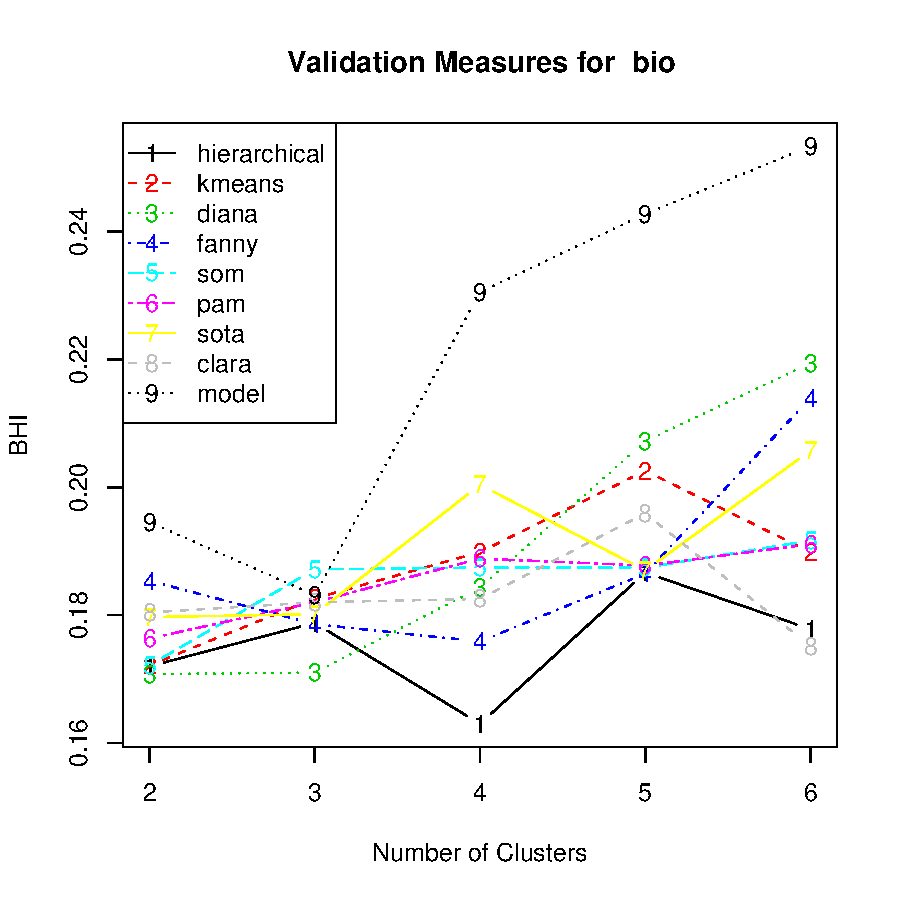
\includegraphics{clValid-015}
  \caption{Plot of the BHI measure, using predetermined functional classes.}
  \label{fig:BHI}
\end{figure}


\begin{figure}
  \centering
\begin{Schunk}
\begin{Sinput}
> plot(bio, measure = "BSI")
\end{Sinput}
\end{Schunk}
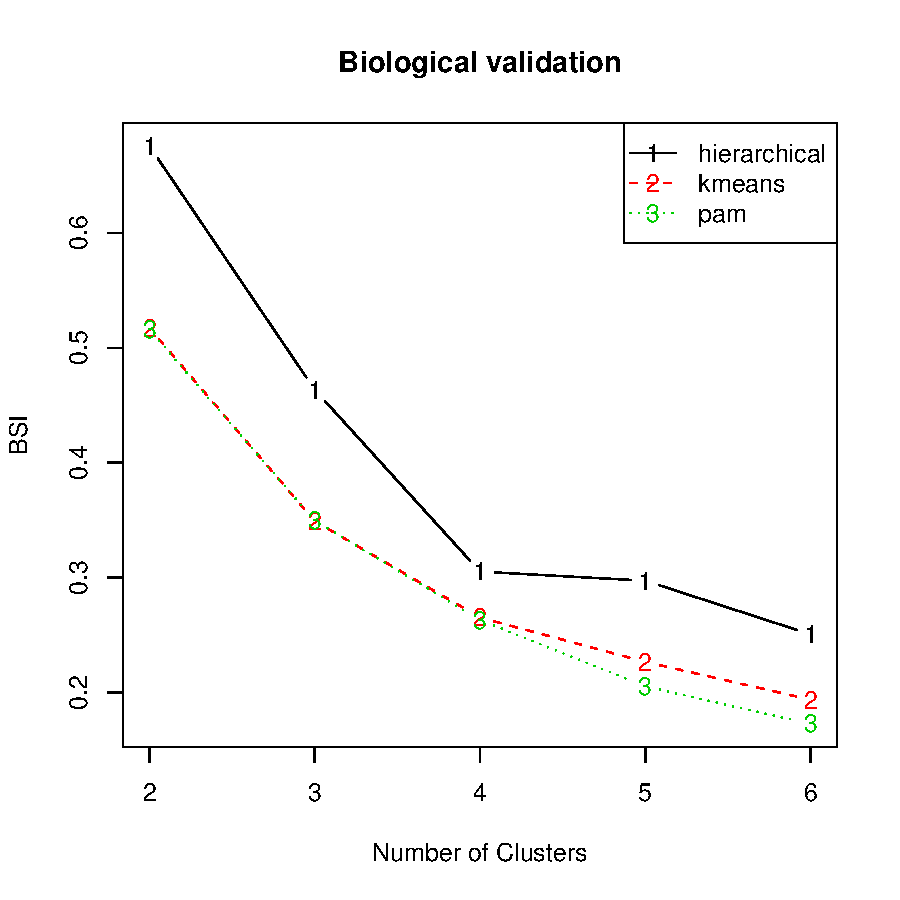
\includegraphics{clValid-016}
  \caption{Plot of the BSI measure, using predetermined functional classes.}
  \label{fig:BSI}
\end{figure}


%Model based clustering appears to have the best BHI score over the
%range for the number of clusters, while hierarchical clustering is
%slightly better than model based overall for the BSI scores.

The other option for biological validation is to use the annotation packages available in
Bioconductor \citep{BioC}.  This option uses the annotation packages
to map the genes to their corresponding GO terms.  There
are three main ontologies, cellular component (``CC''), biological process
(``BP''), and molecular function (``MF''), which can be selected via
the \rfarg{GOcategory} argument.
The user must download, at a
minimum, the \pkg{Biobase}, \pkg{annotate}, and \pkg{GO} packages from
Bioconductor
(\href{http://www.bioconductor.org/}{http://www.bioconductor.org/}),
then load them during the R session.
In addition, any specific annotation packages that are required will need to be downloaded (e.g.,
experiments using the Affymetrix GeneChip hgu95av2 would require the
\pkg{hgu95av2} package).  
Once the appropriate annotation packages are downloaded, they can be
specified in the function call via the \rfarg{annotation} argument.
The \rfarg{goTermFreq} argument is used to select a threshold, so that
only GO terms with a frequency in the dataset above the threshold are
used to determine the functional classes.  

To illustrate, the identifiers in the dataset \ro{mouse} are from the
Affymetrix Murine Genome 430a GeneChip Array, with corresponding
annotation package \pkg{moe430a} available from Bioconductor.  We
leave the \rfarg{goTermFreq} argument at its default level of 0.05,
and use all available GO categories (\rfarg{GOcategory="all"}) for annotation.

\begin{Schunk}
\begin{Sinput}
> if (require("Biobase") && require("annotate") && require("GO") && 
+     require("moe430a")) {
+     bio2 <- clValid(express, 2:6, clMethods = c("hierarchical", 
+         "kmeans", "pam"), validation = "biological", annotation = "moe430a", 
+         GOcategory = "all")
+ }
\end{Sinput}
\end{Schunk}

\begin{Schunk}
\begin{Sinput}
> if (exists("bio2")) optimalScores(bio2)
\end{Sinput}
\begin{Soutput}
        Score       Method Clusters
BHI 0.1372982       kmeans        5
BSI 0.7938518 hierarchical        2
\end{Soutput}
\end{Schunk}

The optimal method and number of clusters for the two measures agree
with those found using the predetermined functional classes, and the   
plots of the measures given in Figures \ref{fig:BHI2} and
\ref{fig:BSI2} are also very similar to the previous plots.
Notice again that hierarchical clustering has the best performance on
the BSI measurement over the range for the number of clusters, 
but does not score as well under the BHI measure validation.  




\begin{figure}
  \centering
\begin{Schunk}
\begin{Sinput}
> if (exists("bio2")) plot(bio2, measure = "BHI", legendLoc = "topleft")
\end{Sinput}
\end{Schunk}
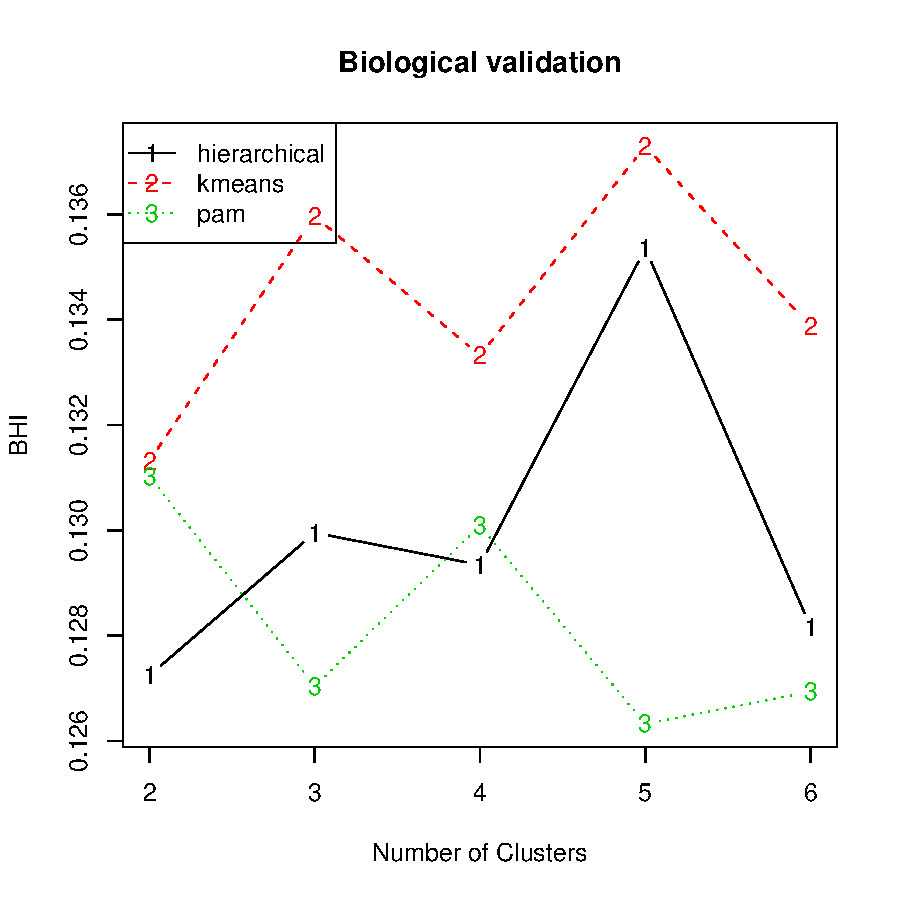
\includegraphics{clValid-021}
  \caption{Plot of the BHI measure, using annotation package
    \pkg{moe430a} in Bioconductor.}
  \label{fig:BHI2}
\end{figure}

\begin{figure}
  \centering
\begin{Schunk}
\begin{Sinput}
> if (exists("bio2")) plot(bio2, measure = "BSI")
\end{Sinput}
\end{Schunk}
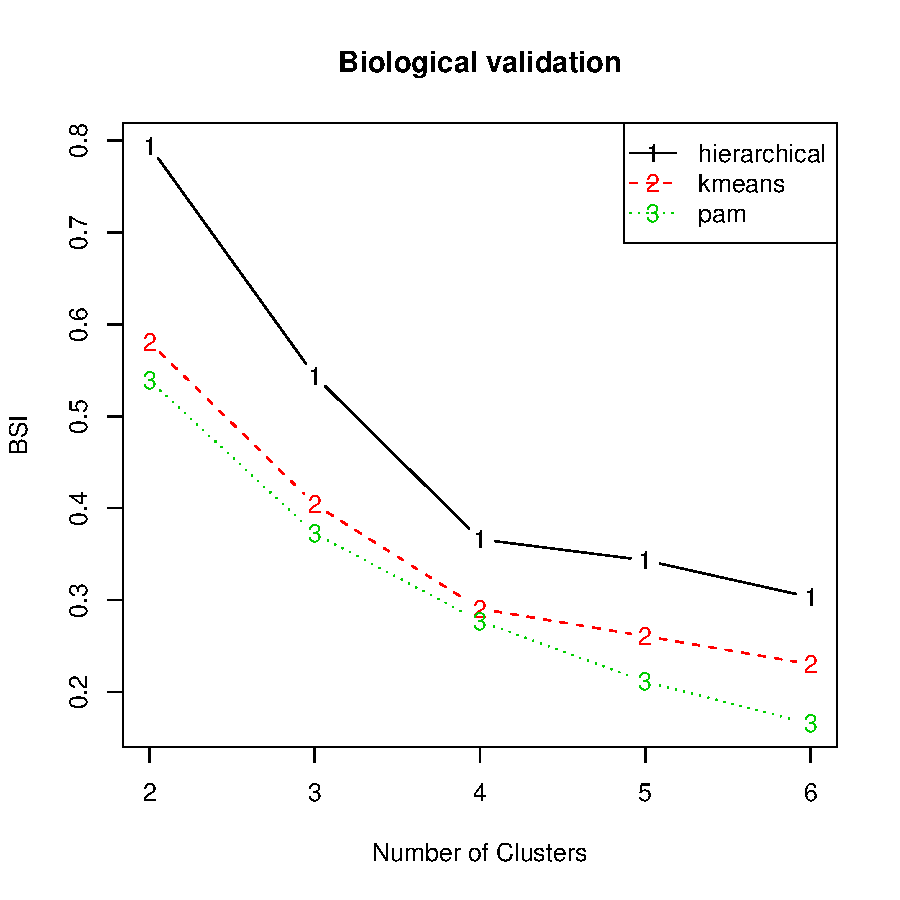
\includegraphics{clValid-022}
  \caption{Plot of the BSI measure, using annotation package
    \pkg{moe430a} in Bioconductor.}
  \label{fig:BSI2}
\end{figure}




\subsubsection*{Further Analysis}

Hierarchical clustering consistently performs well for many of the
validation measures. The clustering results from any method can be
extracted from a \rf{clValid()} object for further analysis, using the
\rf{clusters()} method.  Here, we
extract the results from hierarchical clustering, to plot the
dendogram and view the observations that are grouped together at the
various levels of the topology.  
The dendrogram is plotted in Figure
\ref{fig:hplot}, with the genes belonging to the
``Growth/Differentiation'' (GD) and ``Transcription factor'' (TF) functional
classes labeled. 
The genes belonging to the top two clusters are
cross-classified with their functional annotation given in the
dataset. Of potential interest, the second cluster contains no
genes in the ``EST'' or ``Miscellaneous'' categories.  Further
inspection of the results is left to a subject matter expert.  

\begin{Schunk}
\begin{Sinput}
> hc <- clusters(bio, "hierarchical")
\end{Sinput}
\end{Schunk}

\begin{Schunk}
\begin{Sinput}
> mfc <- factor(mouse$FC, labels = c("Re", "EST", "GD", "KP", "Met", 
+     "Mis", "St", "TF", "U"))
> tf.gd <- ifelse(mfc %in% c("GD", "TF"), levels(mfc)[mfc], "")
> plot(hc, labels = tf.gd, cex = 0.7, hang = -1, main = "Mouse Cluster Dendrogram")
\end{Sinput}
\end{Schunk}

\begin{figure}
  \centering
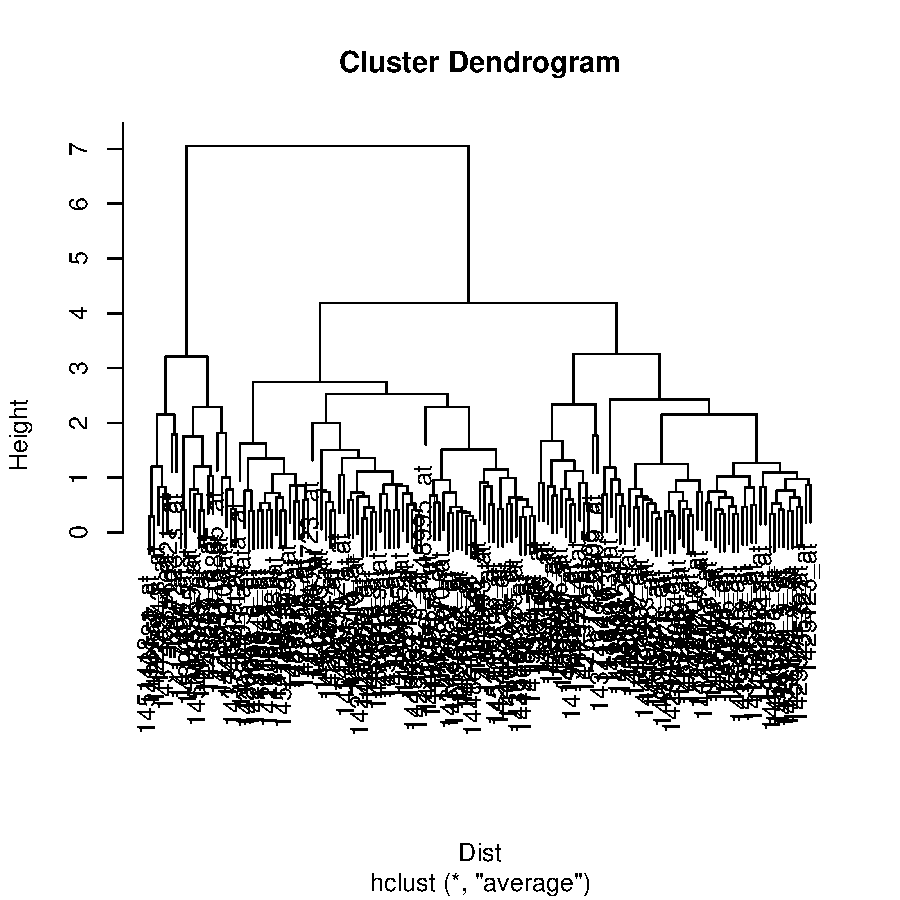
\includegraphics{clValid-025}
  \caption{Plot of the dendogram for hierarchical clustering.}
  \label{fig:hplot}
\end{figure}

\begin{Schunk}
\begin{Sinput}
> two <- cutree(hc, 2)
> xtabs(~mouse$FC + two)
\end{Sinput}
\begin{Soutput}
                        two
mouse$FC                  1  2
  ECM/Receptors          12  4
  EST                    31  0
  Growth/Differentiation 12  4
  Kinases/Phosphatases    4  3
  Metabolism              7  1
  Miscellaneous          25  0
  Stress-induced          4  2
  Transcription factor   23  5
  Unknown                 9  1
\end{Soutput}
\end{Schunk}



\section{Discussion}
\label{sec:discussion}

We have developed an R package, \pkg{clValid}, which contains measures
for validating the results from a clustering procedure.  We categorize
the measures into three distinct types, ``internal'', ``stability'',
and ``biological'', and provide plot, summary, and additional methods
for viewing and summarizing the validation scores and extracting the
clustering results for further analysis.  
In addition to the object-oriented nature of the language, 
implementing the validation measures
within the R statistical programming framework provides the additional
advantage in that it can 
interface with numerous clustering algorithms in existing R packages,
and accommodate further algorithms as they are developed and coded into
R libraries.  Currently, \rf{clValid()} accepts up to ten different
clustering methods.  This permits the user to simultaneously vary the
number of clusters and the clustering algorithms to decide how best to
group the observations in her/his dataset.  Lastly, the package makes
use of  the annotation packages
available in \href{http://www.bioconductor.org/}{Bioconductor} to
calculate the biological validation measures, so that the information
contained in the GO database can be used to assist in the cluster
validation process.


%In microarray analysis, it is common to  cluster both genes and samples
The illustration for the \pkg{clValid} package we have given
here focuses on clustering genes, but it is common in  microarray
analysis to cluster both genes and samples to create a ``heatmap''.
Though the ``biological'' validation measures are specifically
designed for validation of clustering genes, the other measures could
also be used with clustering of samples in a microarray experiment.
Also, for microarray data,  it is a good idea to limit the number of
genes being clustered to a small subset ($100\sim 600$) of the
thousands of expression measures routinely available on a microarray,
both for computational and visualization purposes.  Typically, some
initial pre-selection of the genes based on $t$-statistics,
$p$-values, or expression ratios is performed.

There are several R packages that also perform cluster validation and are available from
\href{http://www.r-project.org}{CRAN} or
\href{http://www.bioconductor.org}{Bioconductor}.   
Examples include the \rf{clustIndex()} function in package \pkg{cclust} \citep{cclust}, which performs 14
different validation measures in three classes,  % ref http://www.wu-wien.ac.at/am/wp99.htm#29
\rf{cluster.stats()} and \rf{clusterboot()} in package \pkg{fpc} \citep{fpc}, the
\pkg{clusterRepro} \citep{clusterRepro} and \pkg{clusterSim}
\citep{clusterSim} packages, and the
\pkg{clusterStab} \citep{clusterStab} package from Bioconductor.  
The \rf{cl\_validity()} function in package \pkg{clue} \citep{clue} does validation
for both paritioning methods (``dissimilarity accounted for'') and
hierarchical methods (``variance accounted for''), and  % ref Journal of Statistical Software (Hornik, 2005b).
function \rf{fclustIndex()} in package \pkg{e1071} \citep{e1071} has several fuzzy
cluster validation measures.  
However, to our knowledge none of these packages offers biological validation or the
unique stability measures which we present here.  \citet{Han2005}
provides C++ code for the validation measures which they discuss, and
the \rf{Caat} tool
available in the \href{http://gepas.bioinfo.cipf.es/}{GEPAS} software
suite offers a web-based interface for visualizing and validating
(using the Silhouette Width) cluster results.  However, neither of
these two tools are as flexible for interfacing with the variety of
clustering algorithms that are available in the R language, or can
automatically access the annotation information which is available in
\href{http://www.bioconductor.org/}{Bioconductor}. 
Hence, the \pkg{clValid} package is a valuable addition to the growing
collection of cluster validation software available for researchers.



{\small
  \bibliographystyle{abbrvnat}
  \bibliography{ClusterRefs}
}


%\bibliographystyle{jss}
%\bibliography{ClusterRefs}




\end{document}


